\documentclass[tikz,border=2pt]{standalone}
% Shared look for the paper's diagrams (built standalone: figures/diagrams/Makefile).
\usepackage[T1]{fontenc}
\usepackage{newtxtext,newtxmath}
\usepackage{xcolor}
\usepackage{tikz}
\usetikzlibrary{positioning,arrows.meta,fit,calc,backgrounds,decorations.pathreplacing}
\definecolor{ink}{HTML}{1F2328}
\definecolor{muted}{HTML}{6A737D}
\definecolor{rulec}{HTML}{D0D4DC}
\definecolor{fillc}{HTML}{F4F5F8}
\definecolor{sone}{HTML}{2A78D6}   % categorical slot 1: Kubernetes Job / trees
\definecolor{stwo}{HTML}{EB6834}   % slot 2: language models
\definecolor{sthree}{HTML}{1BAF7A} % slot 3: combinations
\definecolor{flyte}{HTML}{6250D6}
\tikzset{
  >={Stealth[length=5pt,width=4pt]},
  every node/.style={font=\small, text=ink},
  box/.style={draw=rulec, fill=white, rounded corners=2pt, inner sep=5pt, line width=0.6pt, align=left},
  head/.style={font=\scriptsize\bfseries\sffamily, text=muted},
  note/.style={font=\scriptsize, text=muted, align=left},
  flow/.style={->, draw=muted, line width=0.7pt},
}

\begin{document}
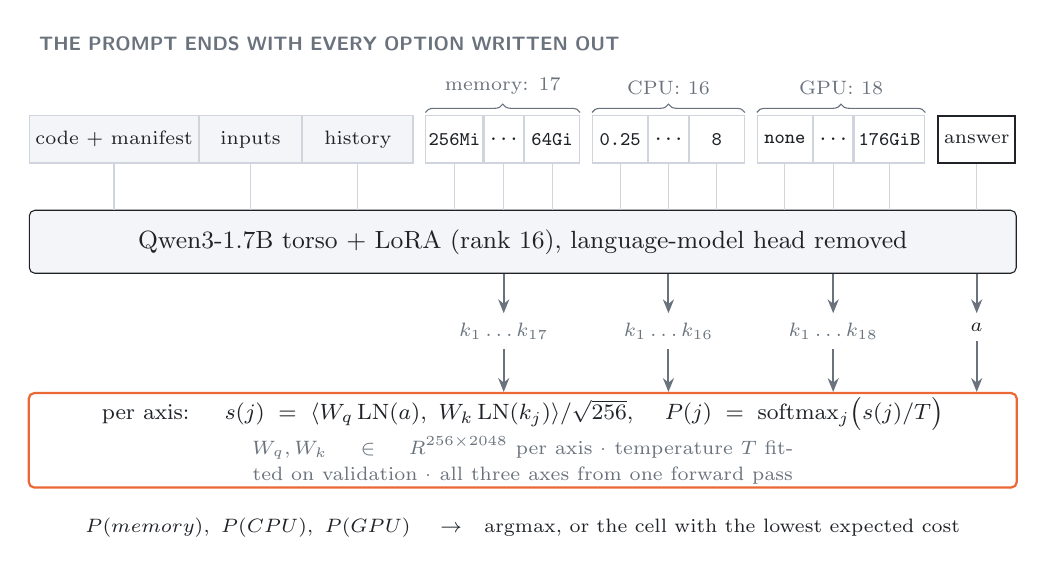
\begin{tikzpicture}[
  tok/.style={draw=rulec, fill=white, minimum height=6mm, inner sep=2pt, font=\scriptsize},
  opt/.style={draw=rulec, fill=white, minimum height=6mm, minimum width=7mm, inner sep=1pt, font=\scriptsize\ttfamily},
]
% the prompt as a row of segments
\node[tok, fill=fillc, minimum width=21mm] (c) at (0,0) {code + manifest};
\node[tok, fill=fillc, minimum width=13mm, right=0mm of c] (i) {inputs};
\node[tok, fill=fillc, minimum width=14mm, right=0mm of i] (h) {history};
\node[opt, right=1.5mm of h] (m1) {256Mi};
\node[opt, right=0mm of m1, minimum width=5mm] (m2) {\ldots};
\node[opt, right=0mm of m2] (m3) {64Gi};
\node[opt, right=1.5mm of m3] (c1) {0.25};
\node[opt, right=0mm of c1, minimum width=5mm] (c2) {\ldots};
\node[opt, right=0mm of c2] (c3) {8};
\node[opt, right=1.5mm of c3] (g1) {none};
\node[opt, right=0mm of g1, minimum width=5mm] (g2) {\ldots};
\node[opt, right=0mm of g2, minimum width=9mm] (g3) {176GiB};
\node[tok, right=1.5mm of g3, minimum width=9mm, draw=ink, line width=0.8pt] (a) {answer};
\draw[decorate, decoration={brace, amplitude=3pt, raise=1pt}, draw=muted] (m1.north west) -- (m3.north east)
  node[midway, above=4pt, note] {memory: 17};
\draw[decorate, decoration={brace, amplitude=3pt, raise=1pt}, draw=muted] (c1.north west) -- (c3.north east)
  node[midway, above=4pt, note] {CPU: 16};
\draw[decorate, decoration={brace, amplitude=3pt, raise=1pt}, draw=muted] (g1.north west) -- (g3.north east)
  node[midway, above=4pt, note] {GPU: 18};
\node[head, above=7mm of c.north west, anchor=south west] {THE PROMPT ENDS WITH EVERY OPTION WRITTEN OUT};

% the torso
\node[draw=ink, fill=fillc, rounded corners=2pt, minimum height=9mm, fit=(c)(a), inner sep=0pt, yshift=-13mm,
      minimum height=8mm] (torso) {};
\node[font=\small] at (torso) {Qwen3-1.7B torso + LoRA (rank 16), language-model head removed};
\foreach \n in {c,i,h,m1,m2,m3,c1,c2,c3,g1,g2,g3,a} { \draw[draw=rulec] (\n.south) -- (\n.south |- torso.north); }

% hidden states at option tokens and the answer slot
\node[note, below=5mm of torso.south -| m2] (km) {$k_1 \ldots k_{17}$};
\node[note, below=5mm of torso.south -| c2] (kc) {$k_1 \ldots k_{16}$};
\node[note, below=5mm of torso.south -| g2] (kg) {$k_1 \ldots k_{18}$};
\node[note, below=5mm of torso.south -| a, text=ink] (qa) {$a$};
\foreach \n in {km,kc,kg,qa} { \draw[flow] (\n |- torso.south) -- (\n.north); }

% the three heads
\path (torso.south west) ++(0,-15mm) coordinate (hl);
\path (torso.south east) ++(0,-15mm) coordinate (hr);
\node[draw=stwo, line width=0.8pt, rounded corners=2pt, fill=white, fit=(hl)(hr), inner sep=0pt, minimum height=12mm,
      anchor=north] (heads) at ($(hl)!0.5!(hr)$) {};
\node[align=center, font=\footnotesize, text width=120mm] at (heads) {per axis: \quad
$s(j) = \langle W_q\,\mathrm{LN}(a),\ W_k\,\mathrm{LN}(k_j)\rangle / \sqrt{256}$, \quad $P(j) = \mathrm{softmax}_j\bigl(s(j)/T\bigr)$\\[1pt]
{\scriptsize\color{muted} $W_q, W_k \in \mathbb{R}^{256\times2048}$ per axis \textperiodcentered\ temperature $T$ fitted on validation \textperiodcentered\ all three axes from one forward pass}};
\foreach \n in {km,kc,kg,qa} { \draw[flow] (\n.south) -- (\n.south |- heads.north); }
\node[note, below=2.5mm of heads, text=ink] {$P(\text{memory}),\ P(\text{CPU}),\ P(\text{GPU})$ \quad$\to$\quad argmax, or the cell with the lowest expected cost};
\end{tikzpicture}
\end{document}
